\section{Design}
In this section, we outline the design of our interactive vowel chart, \visowel{}. We discuss the interface of \visowel{} and its calibration and tutorial, then we present our design of \visowel{}'s signal processing backend.

\subsection{User Interface}
\visowel{} is comprised of a vowel chart, which displays the Spanish speaker's and user's vowels, recording buttons, and audio playback button for the Spanish speaker. When any vowel is clicked, including the Spanish speaker's, audio plays. In order for \visowel{} to display two speakers on one chart, the user must first have their voice calibrated. Once their voice is calibrated, users are able to complete a tutorial introducing them to \visowel{} where they practice with English words and Spanish words to begin to build mental models of how it works. 

\begin{figure}[t]
    \centering
    \begin{subfigure}{\linewidth}
        \centering
        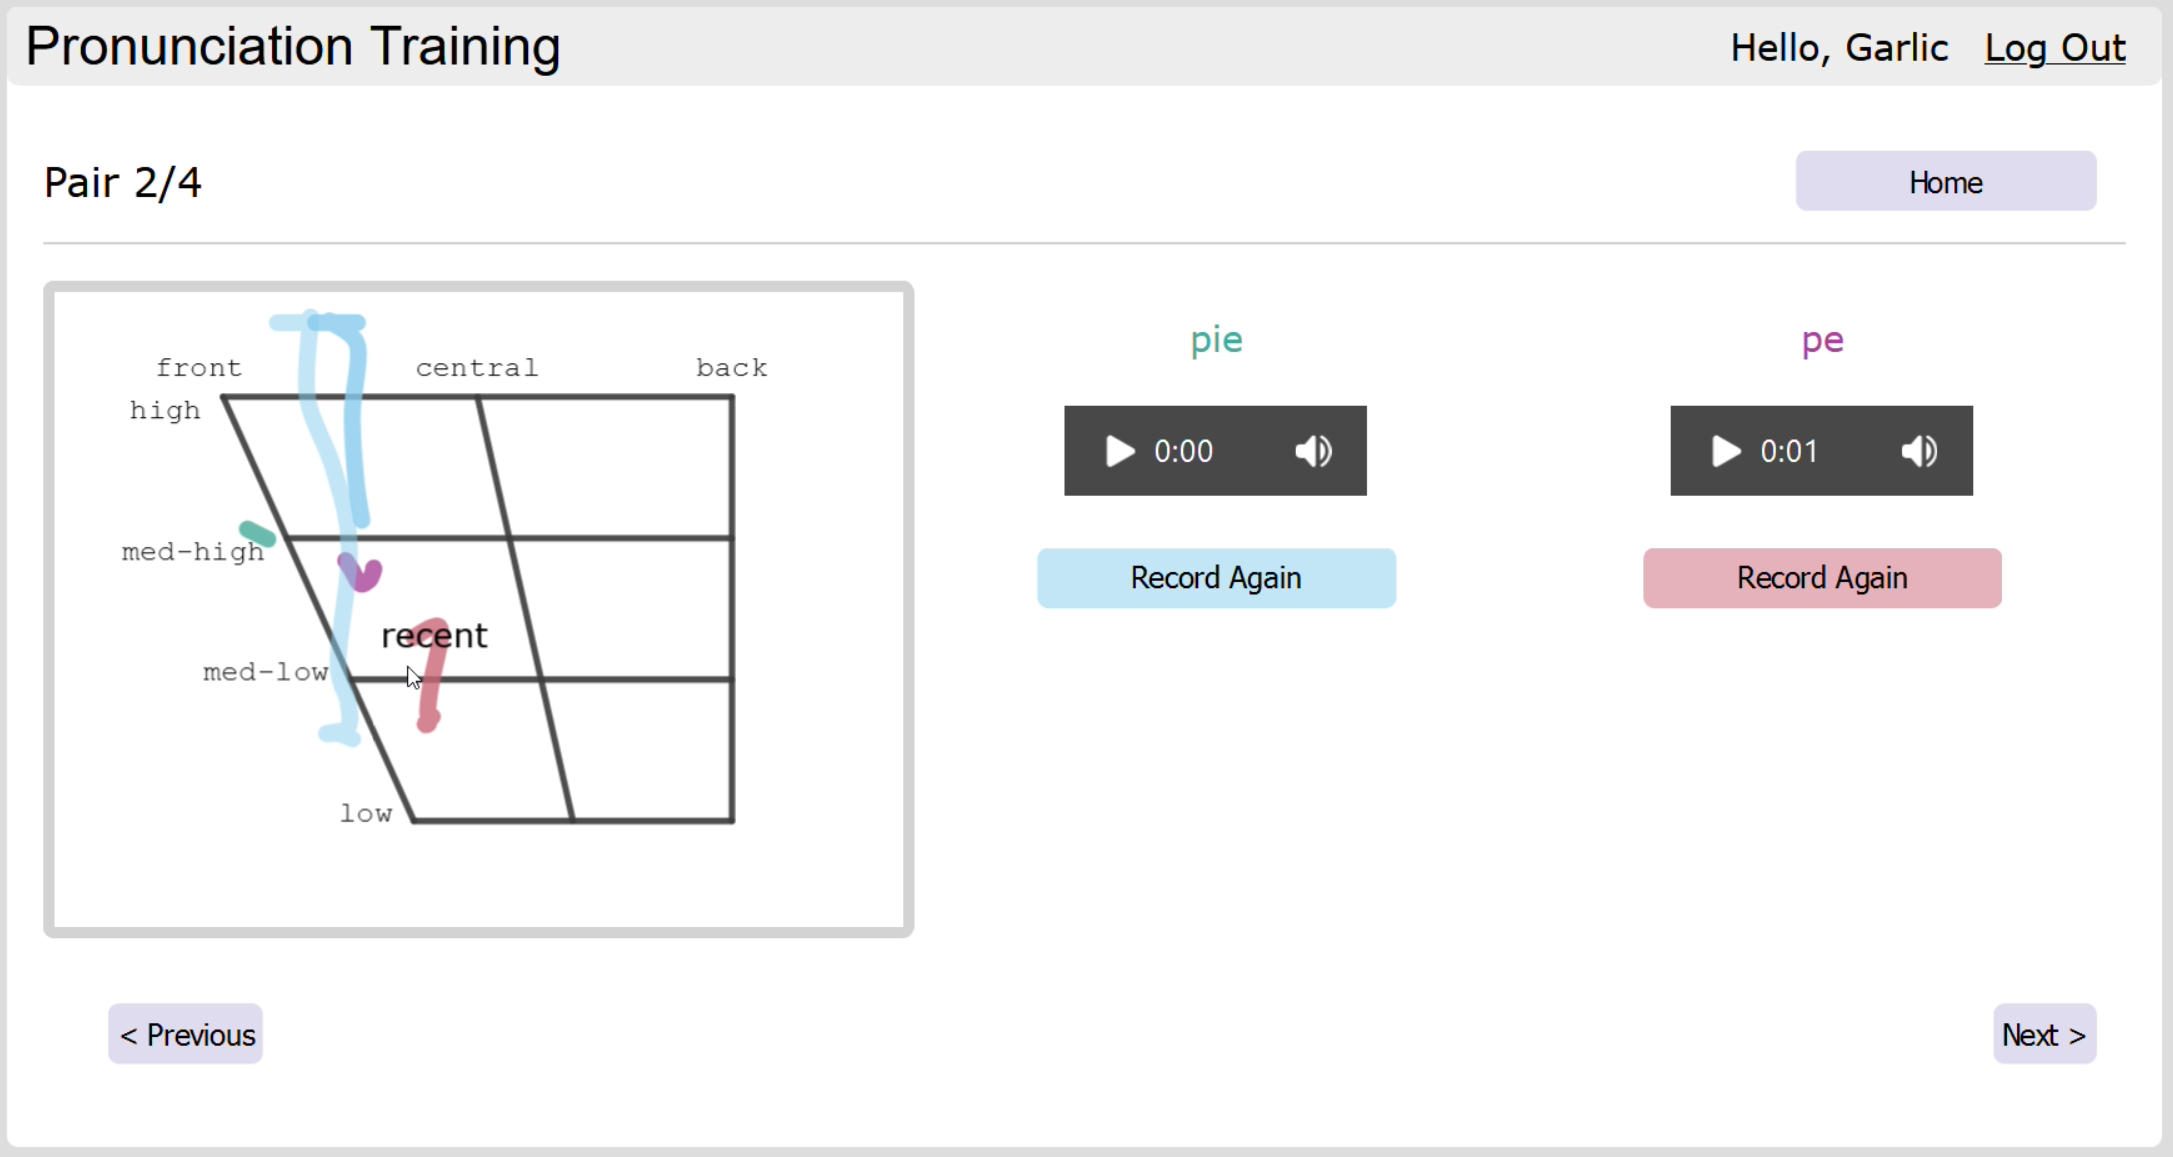
\includegraphics[width=\linewidth]{pictures/practice/visowelPractice.png}
        \caption{A practice page for \visowel{}. The user has recorded twice for "pie" and once for "pe". The most recent recording is "pe". }
        \label{fig:visowelPrac}
    \end{subfigure}
    \newline
    \begin{subfigure}{\linewidth}
        \centering
        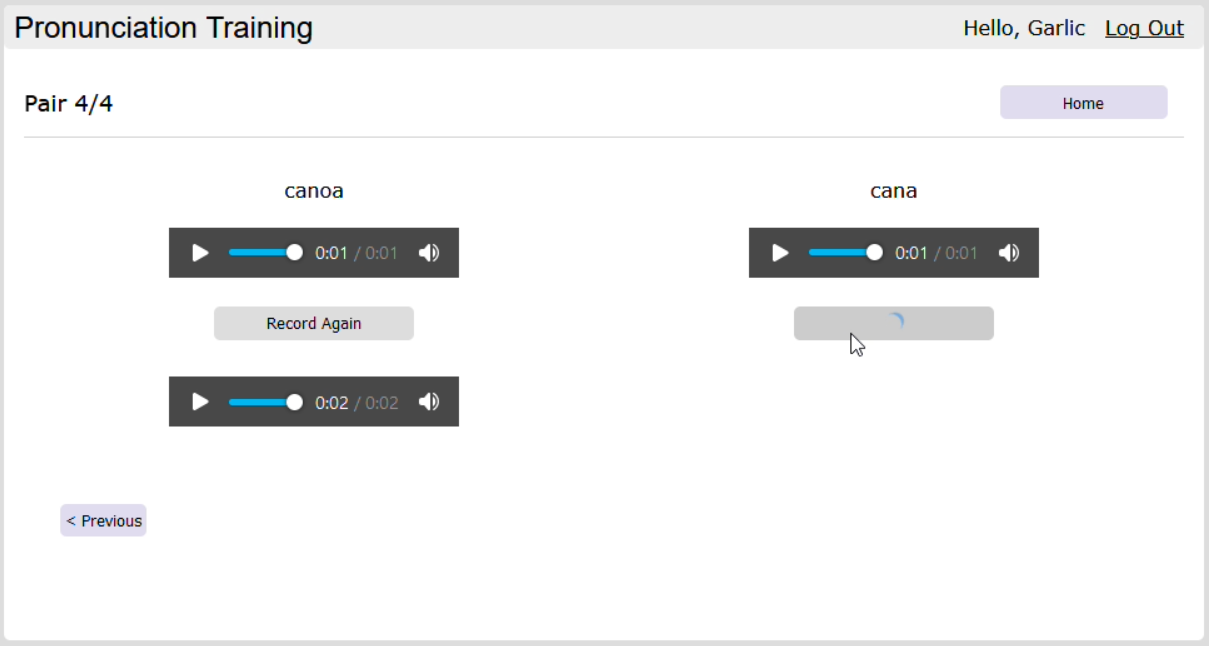
\includegraphics[width=\linewidth]{pictures/practice/audioOnlyPractice.png}
        \caption{A practice page for audio-only. The user is waiting to record "cana", as shown by the semi-circle in the record button.}
        \label{fig:audioPrac}
    \end{subfigure}
    
    \caption{Example practice pages from audio-only and \visowel{}.}
    \label{fig:pracPages}
\end{figure}


\begin{figure}
    \centering
    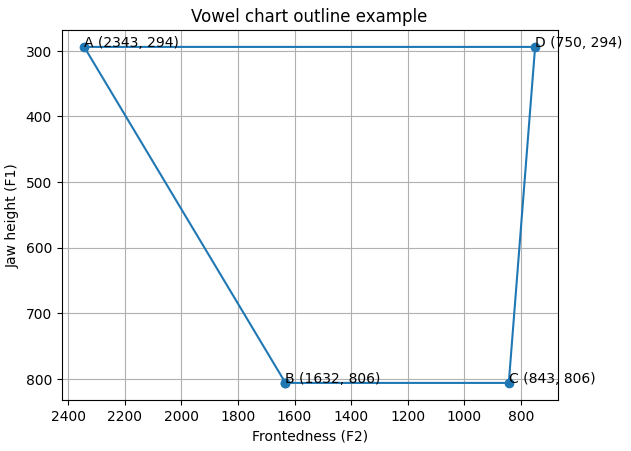
\includegraphics[width=1\linewidth]{pictures/vowel_chart_initial.png}
    \caption{A vowel chart with first and second formant frequency markings.}
    \label{fig:freqVwlChart}
\end{figure}
% Calibration first
% 
\subsubsection{\visowel{}} 
The final design of \visowel{} is trapezoidal shaped and has descriptive labels on the top and left sides, e.g. front, mid, back, etc. Both of these design decisions were inspired by a traditional vowel chart (Figure \ref{fig:exampleVwlChart}). 

\paragraph{Vowel lines.} Vowels are plotted on the chart based on their change in frequencies over time. Clicking on a plotted vowel plays the associated audio for the extracted vowel then the whole word. If the vowel moved over time, an animation redraws the line starting from the beginning. Initially, we attached a simple arrow on the end of the line to indicate vowel change direction (Figure \ref{fig:manyRecordings}). The arrowhead helped, but due to changes in formants, it would sometimes point the wrong direction on the line. In the final version, we removed the arrowhead and added an animation of the line when it was clicked to communicate change over time. 

The vowel trajectory is based on averaging neighboring formants. We began by directly plotting all extracted formant values but since extracted formants vary slightly, this created noisy lines. Because the difference in neighboring formants is due to slightly inaccurate formant extraction and not a speaker's tongue movement, we decreased the visual noise by averaging neighboring formants. 

\paragraph{Multiple recordings.} A user can record words as many times as they would like, however, only the most ten most recent recordings are displayed on the chart. Each time a new vowel is plotted on the chart, the previous vowels become more transparent. In the beginning phases of design, we did not limit the number of vowels on the chart nor the number of vowels extracted from the word (Figure \ref{fig:twoVowels}). The mock-up tested well, but practically, plotting even one vowel proved visually overwhelming when the vowel was long, did not stay in the same place, or was recorded more than a few times. Many recordings created visual clutter on the chart, so we limited the total number of recordings to ten per word and use opacity to communicate the ordering of recordings.

\paragraph{Grid lines and labels.} In our first design, we followed previous work and marked frequencies along the axes (Figure \ref{fig:freqVwlChart})~\cite{rehman2021real,paganus2006vowel}. Discussion with the pretest group showed that people were unsure how to interpret vowels marked on the chart. Our research team decided to strip a vowel chart from all labels, then reintroduce labels one at a time to gauge understanding of the chart based on available labels. Frequency labels did not allow group members to understand what that meant with respect to their physical movements while physical labels (front, back, high, low) were more helpful in interpretation.

Although \visowel{} has bounding grid lines, vowels are not constrained to them. When we forced vowels within the trapezoid, crucial information was lost regarding the current tongue position with respect to previous recordings (Figure \ref{fig:manyRecordings}). For example, the vowel "ea" ([i]\footnote{Square brackets around a character indicate a phonetic description.}) in the English word "beat", could be plotted as slightly above or further forward than the previous recordings, which would put it outside the chart. Removing this information would inaccurately represent the tongue's position as the same between two recordings even though it had moved. As a result, we let vowels be plotted outside the chart. We kept vowels within a wider box around the grid lines, so that even if our extraction algorithm failed to pick out the correct frequencies for the formant, users would have visual feedback.



\begin{figure}[t]
    \centering
    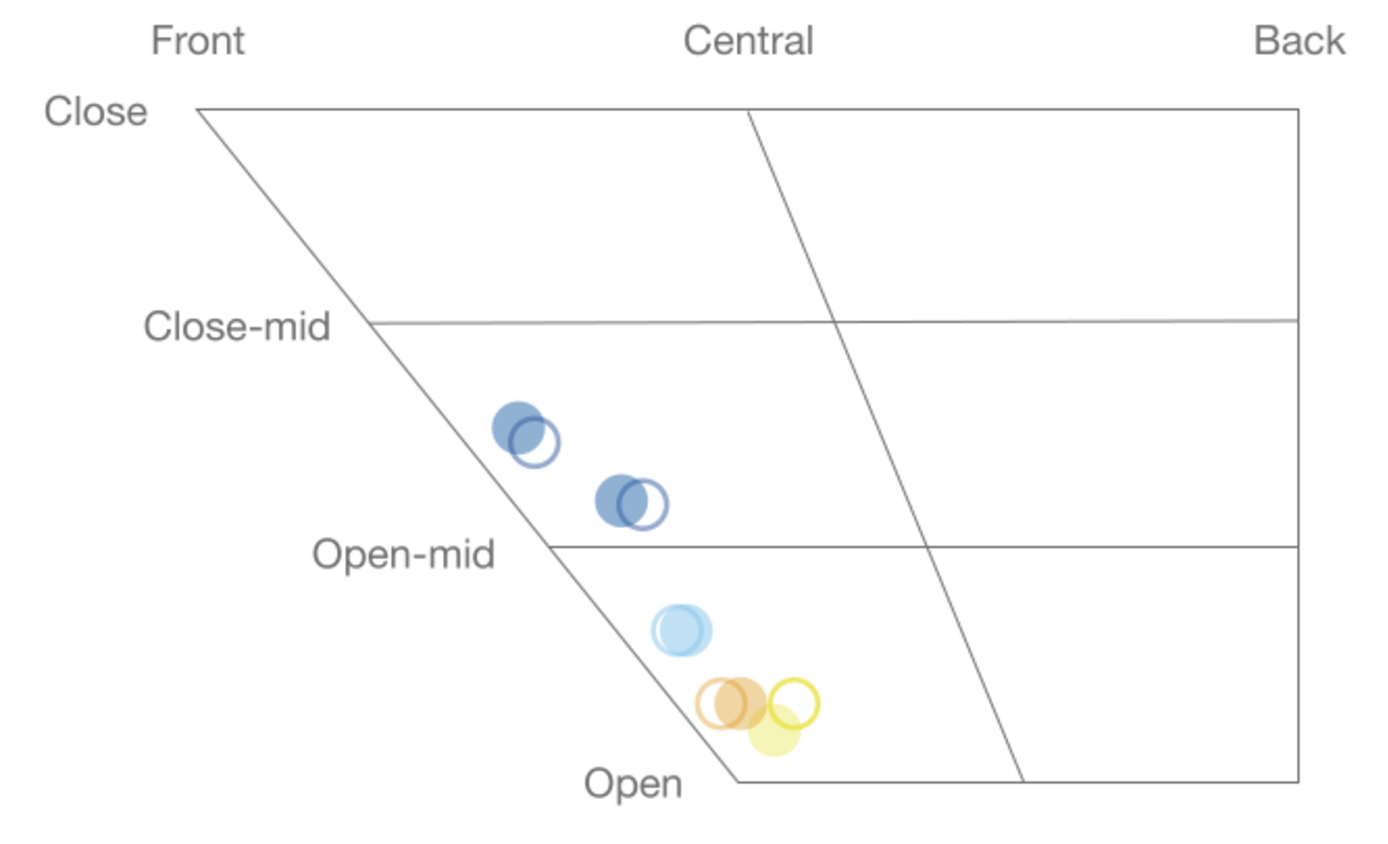
\includegraphics[width=0.65\linewidth]{pictures/vowel_charts/mockup_vwl.pdf}
    \caption{A mock-up of two vowels from one word plotted on a vowel chart. The first vowel's dot is colored in and the second vowel's dot is outlined. }
    \label{fig:twoVowels}
\end{figure}



% Once recording starts, the interface displays a spinning circle for 0.5 seconds to allow the speech recognition algorithm to establish a noise threshold, then recording bars replace the circle. Once the speaker has stopped speaking, the algorithm extracts the vowel boundaries (onset and offset times) and formants of the vowel. Initially, we used written feedback, \textit{"Please wait..."}, that would appear after a user pressed record. Pretests revealed that users would immediately speak as soon as they pressed "Record", only later realizing that the text asked them to wait. When we switched to the spinning symbol, further tests showed that the change caused the users to pause until recording bars appeared. 

\begin{figure}[t]
    \centering
    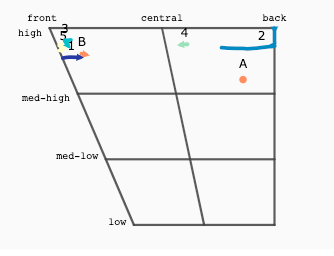
\includegraphics[width=0.85\linewidth]{pictures/vowel_chart_numbered.png}
    \caption{\visowel{} with Spanish vowels marked by A and B and user's vowels labeled numerically with the latest recording starting at 1.}
    \label{fig:manyRecordings}
\end{figure}


\begin{figure}[t]
    \centering
    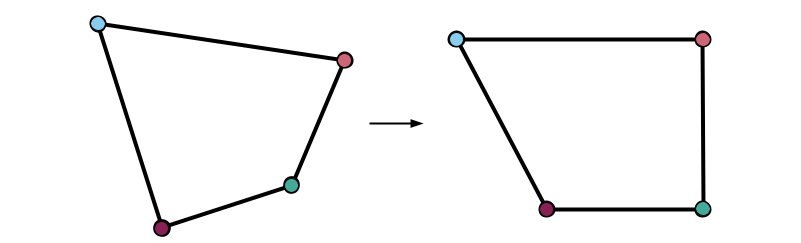
\includegraphics[width=0.45\textwidth]{pictures/transform.png}
    \caption{On the left is an example frequency shaped trapezoid using corner vowels. We use a projective transformation to map  the observed formant frequencies and to a consistent vowel chart representation.}
    \label{fig:transform}
\end{figure}
% \paragraph{\textbf{Calibration}}
% Before a user can interact with \visowel{}, their voice is transformed from the frequency domain into the SVG domain. The transformation comes from a learner's elicitation of the English "corner" vowels, [i,u,\ae,\textturnscripta(6)] extracted from the words beet, boot, bat, and bought. By basing each transformation on a specific speaker's vowels, visualizations more closely represent human perception of sounds by removing speaker-unique characteristics and retaining language-dependent features (Figure \ref{fig:transform}).

\paragraph{\textbf{Calibration}} User voices can vary significantly depending on the individual. This variety will change the shape of the vowel space per individual, as shown by the left image in Figure \ref{fig:transform}. We transform the individual vowel space into a fixed trapezoid, as shown by the right image in Figure \ref{fig:transform}, which removes idiosyncratic speech characteristics and retains language-dependent features. We collect the user's specific vowel space using their elicitation of the English "corner" vowels, [i,u,\ae,\textturnscripta(6)] extracted from the words beet, boot, bat, and bought. We use projective transformation (homography) to map the user-specific frequencies to our vowel chart. Since there is no set ratio for vowel chart trapezoids, we chose the trapezoid ratio for height, top width, and bottom width as 1, 1.33, and 0.833 respectively. The height represents the spread of the first formant ($f_1$) frequency, and the width represents the spread of the second format at different $f_1$. This shape is consistent with the known spread of the vowel chart. The consistent shape of the vowel chart enhances the aesthetics of the chart and the interpretability of results across users.

%% Talk about the mathematics of the process

\paragraph{\textbf{Tutorial}} 
The tutorial for \visowel{} leads learners through understanding a vowel chart. It introduces the tongue's position for producing vowels, how to understand the axes of the vowel chart, and finally, how to mimic a speaker based on their plotted vowel. We settled on this flow based on pretest user interaction with paper and interactive prototypes (details in Appendix \ref{app:tutorial}). We begin with informing users of the tongue's role in producing a vowel, specifically focusing on closeness to the roof of the mouth, tongue height, and where it is in the mouth, close to the teeth or away. We started with the tongue's position, since pretest users were not sure how the tongue's position related to vowel production. After an overview of the chart in relation to tongue position, we give them opportunities to focus on pairs of English vowels that differ in tongue position and height. By starting with known vowels, we were able to bake interaction into the examples and avoid a lot of written instruction, since pretest users often skipped reading.

\begin{figure}[h]
    \centering
    \begin{subfigure}{\linewidth}
        \centering
        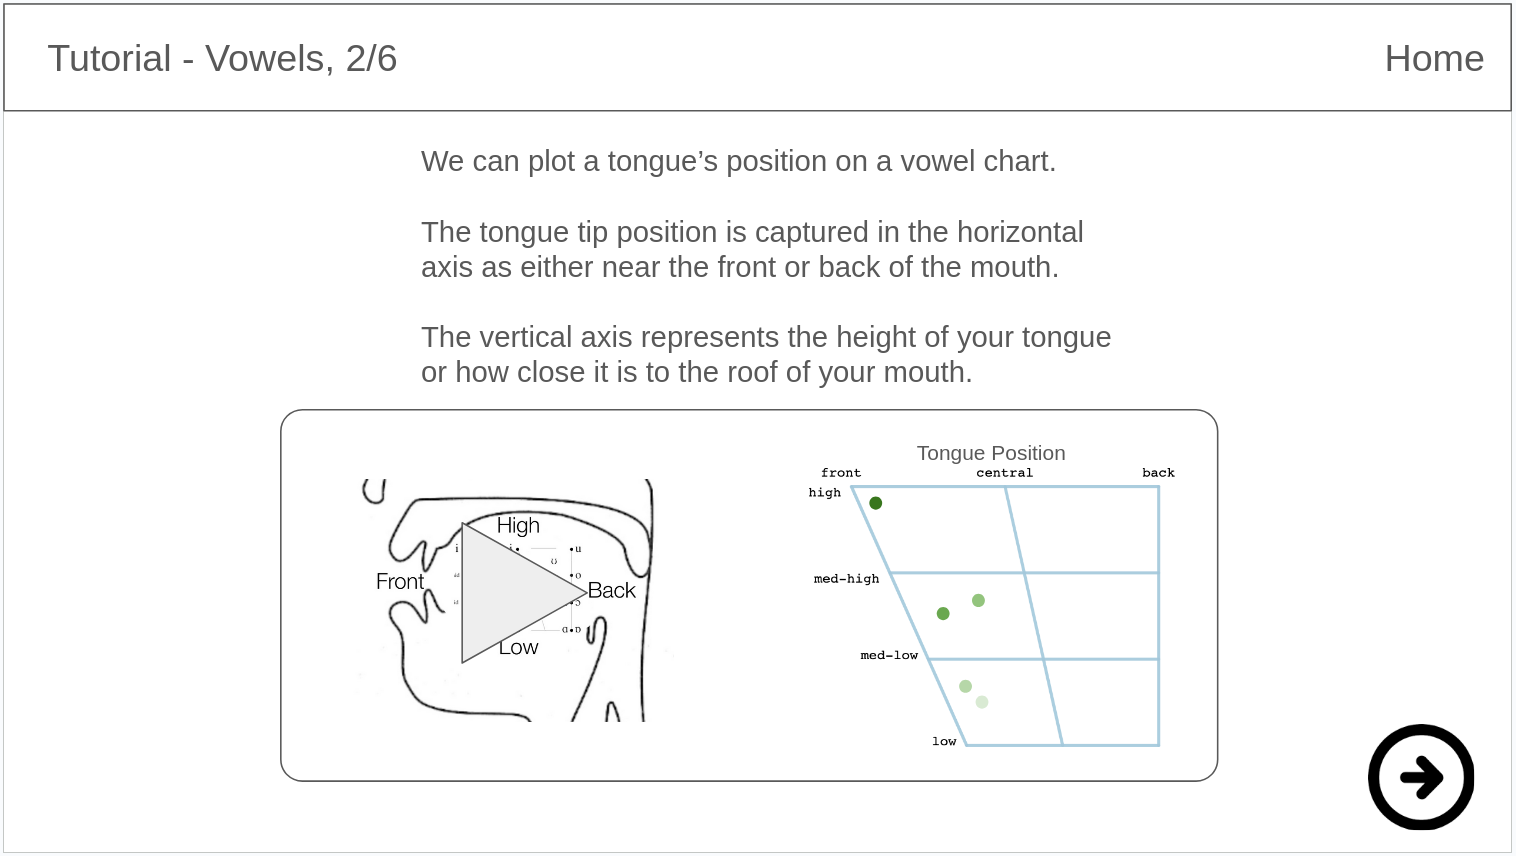
\includegraphics[width=0.9\linewidth]{pictures/tutorial/tut2paper.png}
        \caption{The second page of the paper prototype. One face cutaway is on the left and on the right a vowel chart has multiple different vowels plotted on it.}
        \label{fig:2tutPaper}
    \end{subfigure}
    \begin{subfigure}{\linewidth}
        \centering
      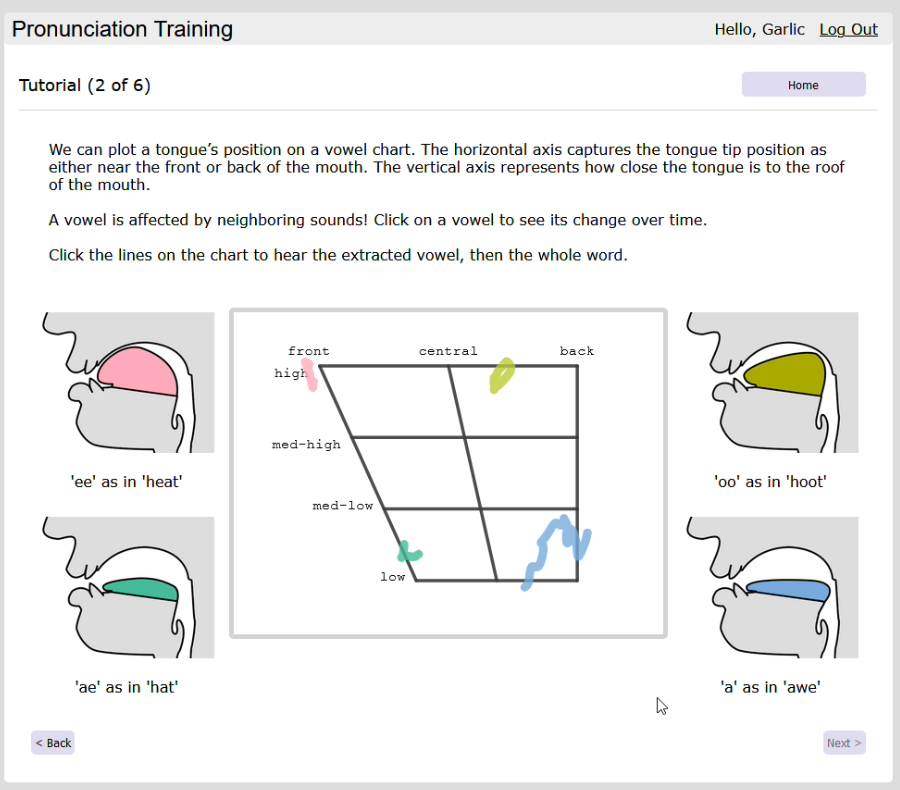
\includegraphics[width=0.825\linewidth]{pictures/tutorial/tut2.png}
        \caption{Final interface for the tutorial's second page. The vowels on the chart share the same color as the tongue in their respective face cutaway.}
        \label{fig:2tut}
    \end{subfigure}
    \label{fig:pg2}
    \caption{Design cycle of page 2}
\end{figure}

\subsection{Technical Backend}
\begin{figure*}[ht]
    \centering
    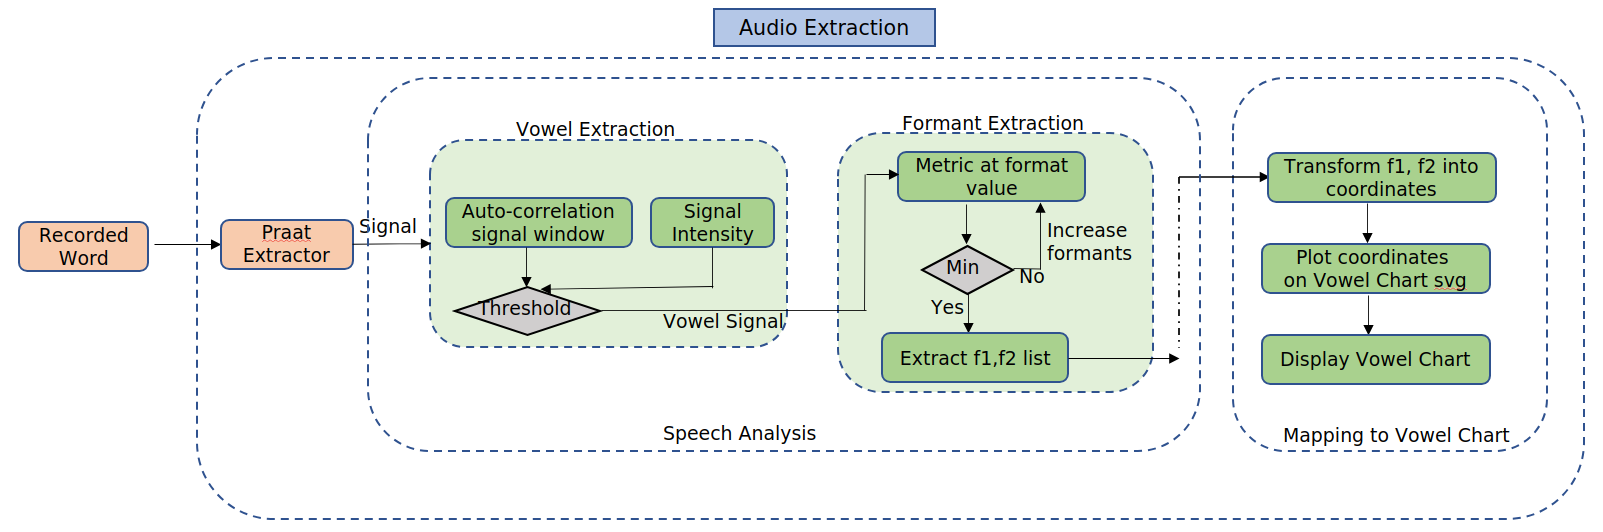
\includegraphics[width=\linewidth]{pictures/workflows/extractionAudio.png}
    \caption{A flowchart representing the algorithmic process of extracting vowels and formants. }
    \label{fig:extractAudio}
\end{figure*}
We discuss the design of the signal processing algorithm and its accuracy based on pre-study results. The algorithm extracts the vowel and vowel formants, then transforms the formants into the html viewbox according to a speaker's transformation (Figure~\ref{fig:extractAudio}). An audio file with a single word is passed as a signal to the vowel extractor. The vowel extraction uses the autocorrelation of the signal to determine the onset and offset times of the vowel. A ".wav" file is created using these timestamps. The new file is passed into formant extraction which tests different numbers of formants and calculates a goodness metric. The algorithm extracts $f_1$ and $f_2$ values using the formant with the best metric. The lists of $f_1$ and $f_2$ are transformed into the viewbox then displayed on the vowel chart. 

\subsubsection{Vowel Extraction}
\begin{figure}[t]
    \centering
    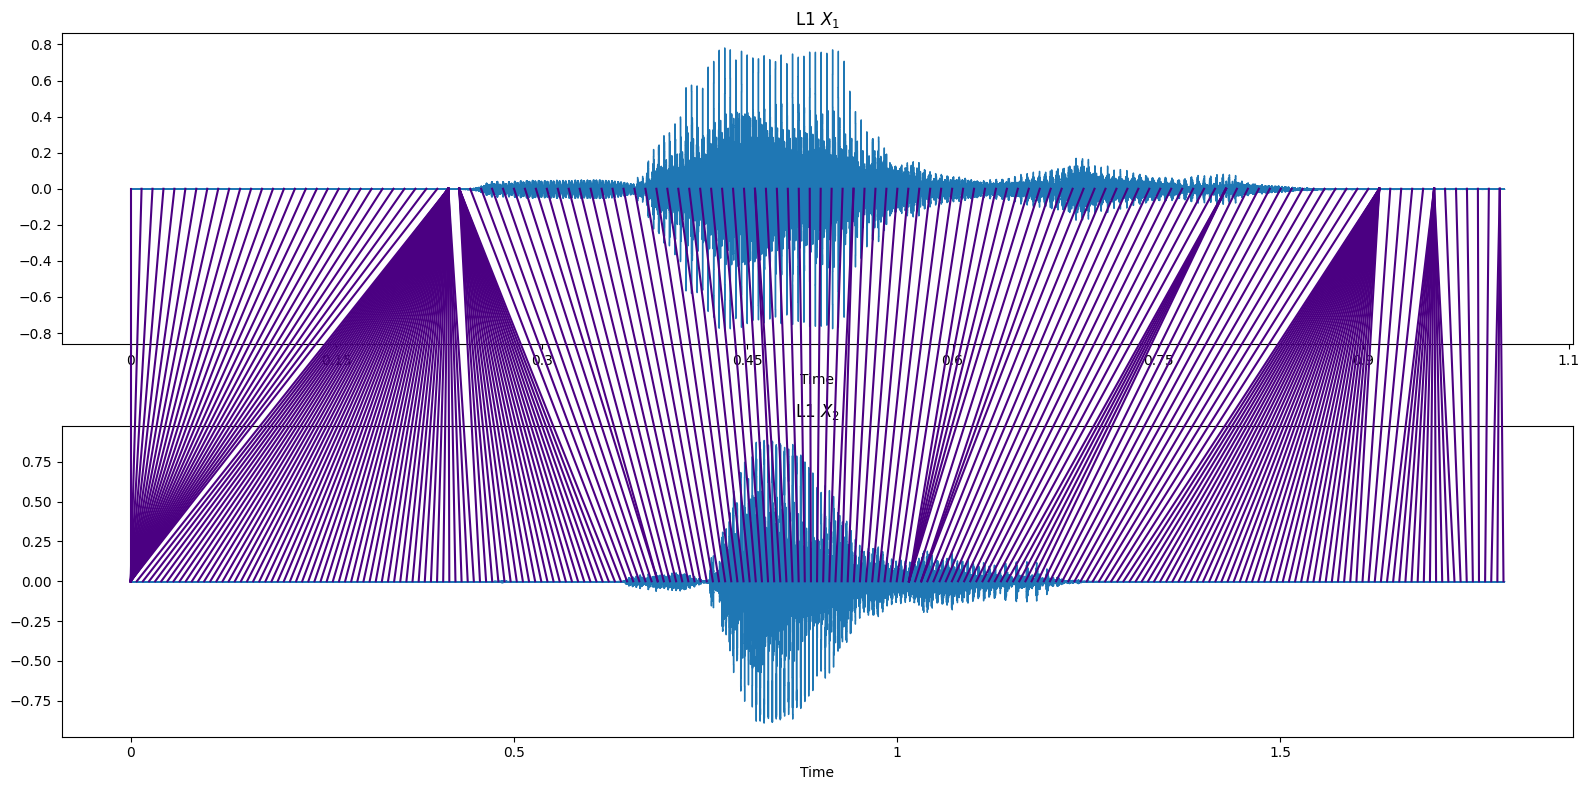
\includegraphics[width=\linewidth]{pictures/DTW.png}
    \caption{An example graph we made demonstrating the Dynamic Time Warping (DTW) algorithm~\cite{bellman1959dtw} which matches similar parts of two different signals. The purple lines represent the connections DTW made.}
    \label{fig:DTW}
\end{figure}
We designed a vowel extraction algorithm based on the autocorrelation of the signal after testing two existing algorithms that did not have the precision needed, Dynamic Time Warping (DTW)~\cite{bellman1959dtw} and PocketSphinx Phoneme Aligner (PS)~\cite{huggins2006pocketsphinx}, as shown in Table \ref{tab:algoTimes}. We tested the algorithms on 5 voices from our lab, 3 female. Even though DTW generally had a lower absolute difference, it tended to mark the beginning of the vowel during the consonant, as represented by the negative. We determined the precision needed through trial and error. Starting 20 milliseconds after the expected beginning of the vowel will not miss diphthong information but starting more than 10ms before the start of the vowel will pick up on too much of the preceding consonant vice versa for vowel offset. 

\begin{figure}[ht]
    \centering
    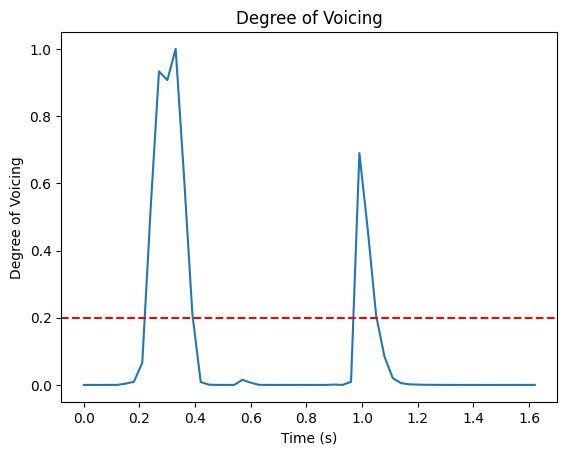
\includegraphics[width=\linewidth]{pictures/dtwThreshold.jpeg}
    \caption{An example degree of autocorrelation for the word 'bata' of a signal with the threshold marked horizontally in red. The two peaks are the vowels.}
    \label{fig:extractAudio}
\end{figure}

Our novel signal processing algorithm extracts the beginning and end of the vowel by calculating the degree of autocorrelation within a sliding window, where autocorrelation is computed as follows:

\begin{align*}
    c_k = \sum_n v_{n+k} \cdot \overline{v}_n
\end{align*}

where $v$ is the audio signal and $\overline{v}_n$ is the complex conjugate.  
Once the autocorrelation goes over a predefined threshold and then back under, the code marks the timestamps (Figure \ref{fig:extractAudio}). We set the threshold by experimenting on different words and speakers to find the degree of autocorrelation needed to be considered a vowel. This algorithm produced the most accurate timestamps for the beginning of the vowel though it still produced inaccurate endings based on whether the following consonant was also fairly resonant. 

\begin{table}[!ht]
    \centering
    \begin{tabular}{ll}
        Algorithm & Average diff. to Manual Calculation \\ \hline
        DTW & -8.2ms \\ 
        sphinx & 25.4ms \\ 
        Ours & 13.4ms \\ 
    \end{tabular}
    \caption{The average difference in onset times for three vowel extraction algorithms. We ended with ours because it was better to lag than lead the beginning of the vowel}
    \label{tab:algoTimes}
\end{table}

% \subsubsection{formant extraction}

% \todo{Dipayan:}
% We used Praat's formant extraction which requires a frequency ceiling and number of formants. Because the number of formants in a signal changes based on word not speaker, we tested formants extracted using 4, 5, and 6 formants. 
%  \begin{align*}
%      metric &= std (value) \\
%      out method &= do this \label{eq:1}
%  \end{align*}

% We measured the standard deviation (std) across the frequencies and the degree of overlap between the first and second formants. The lower std and lower degree of overlap that a formant has the greater the likelihood that the algorithm found the correct frequencies for the first and second formant. 

\subsubsection{Formant Extraction.}
We use Praat's ~\cite{hugoQuenePraat} format extraction library to retrieve the first two formants. Praat's method requires a frequency ceiling and the number of formants.  We set the frequency ceiling at 5500 Hz. However, since the number of formants in a signal changes based on the word, not the speaker, we designed a metric for a signal, described below, to measure the best formant for the signal. We need the first two formants to be smooth because when the algorithm incorrectly chooses a formant, the formant tends to jump multiple frequencies between points.

 \begin{align*}
     &\textit{smoothness}(sig) = stddev(sig) \\
     &metric(sig,fmt\_cnt) =  \textit{smoothness}(sig_{f1}) + \textit{smoothness}(sig_{f2})\\ &\quad \quad \quad \quad \quad \quad \quad \quad \quad + \sum_{i=3}^{fmt\_cnt} 0.8^{i-2} \textit{smoothness}(sig_{fi})
 \end{align*}

Based on this metric, we choose the formant number which has the lowest metric value. It ensures that the first two formants are consistent for the signal, and the higher formants are also somewhat stable. The stability of the formant ensures that our algorithm has found the correct frequency for the first and second formant.